
\documentclass[12pt]{article}
%\usepackage{blindtext}
\usepackage{listings}
\usepackage{tikz}
\usepackage{graphicx}
\graphicspath{{./images/}}
\usepackage{eurosym}
\usepackage{textcomp}
\usepackage{afterpage}
\usepackage{hyperref}
\usepackage{listings}
\usepackage{amsfonts}
\usepackage{sectsty}
\usepackage{multicol}
\usepackage[margin=1cm]{caption}
\usepackage{tabu}
\usepackage{array}
\usepackage[trim]{tokenizer} 

\newcounter{sncolumncounter}
\newcounter{snrowcounter}

\def \nodelabel#1{%
\setcounter{snrowcounter}{1}
 \foreach \i in {#1}{%
   \draw (\value{sncolumncounter},\value{snrowcounter}) node[anchor=south]{\i};
   \addtocounter{snrowcounter}{1}
 }
 \addtocounter{sncolumncounter}{1}
}

\def \nodeconnection#1{%
  \foreach \i in {#1}{%
    \GetTokens{nodesrc}{nodedest}{\i}
    \draw (\value{sncolumncounter},\nodesrc) node[circle,fill=black]{}--(\value{sncolumncounter},\nodedest) node[circle,fill=black]{};
  }
  \addtocounter{sncolumncounter}{1}
}
 
\newenvironment{sortingnetwork}[3]
{
  \setcounter{sncolumncounter}{0}
  \def \sn@fullsize{15}
  \begin{tikzpicture}[scale=#3*\sn@fullsize/10]
  \foreach \i in {1, ..., #1}
  {
    \draw (0,\i)--(7-1,\i);
  }
}
{
  \end{tikzpicture}
}


\lstset{
   basicstyle=\fontsize{9}{10}\selectfont\ttfamily
}
\newcommand\blankpage{%
    \null
    \thispagestyle{empty}%
    \addtocounter{page}{-1}%
    \newpage}

\newenvironment{tightcenter}{%
  \setlength\topsep{0pt}
  \setlength\parskip{0pt}
  \begin{center}
}{%
  \end{center}
}

    
\allsectionsfont{\raggedright}


\begin{document}

\afterpage{\blankpage}

\begin{titlepage}

\begin{center}

UNIVERSITATEA "ALEXANDRU IOAN CUZA" DIN IAȘI
\\
\textbf{Facultatea de Informatica din Iasi}
\end{center}

   \vspace{20mm}

\begin{center}
    \end{center}
   \vspace{10mm}
\begin{center}
	\Large{LUCRARE DE LICENTA}\\
	
	\vspace{10mm}
	
	\large \textbf{CREARE RETELELOR DE SORTARE FOLOSIND DEEPLEARNING}\\
	\vspace{5mm}
		
	\vspace{5mm}
	\large\textit {DANILA MARIUS CRISTIAN}
	\\
	\vspace{20mm}
	\textbf{Data: }\textit{Iulie, 2018}\\
	\vspace{10mm}
	\textbf{Coordonator}\\
	\textbf{\textit{Lect. Dr. Frasinaru Cristian}}
	\vspace{30mm}
\end{center}
\end{titlepage} 

\definecolor{light-gray}{gray}{0.95}
\renewcommand{\refname}{Bibliografie}  % for the article class
\renewcommand{\contentsname}{Cuprins}
\renewcommand{\figurename}{Fig.}
\newcommand{\code}[1]{\colorbox{light-gray}{\texttt{#1}}}

\begin{abstract}

Scopul acestei lucrari este de a construi un algoritm de deeplearning care sa genereze compartorii dintr-o retea de marime $N$. $N$ reprezinta numarul de fire din retea.
Desi exista abordari neimperative functionale, care genereaza rezultate intr-un timp multumitor, nu s-a mai incercat pana acum generarea de retele de sortare prin aceasta abordare. Rezultatul obtinut este un model antrenat care produce rezultate pentru retele de dimensiuni mici.

\tableofcontents

\end{abstract}

\vspace{80mm}

\pagebreak

\section{Introducere}

O retea de sortare reprezinta un model abstract din informatica, compus din fire si comparatori. Scopul comparatorilor este de a interschimba 2 numere de pe firele pe care sunt plasati. Desi sunt modele simple, retelele de sortare au aplicatii numeroase in calculul paralel si sunt folosite la sortarea seturilor de numere in cadrul placilor grafice.
 
   In cadrul acestei lucrari mi-am propus sa dezvolt un model capabil sa genereze, pe baza unui numar $N$ de fire primit ca input, lista de comparatori necesari pentru o retea de sortare cu $N$ fire. In cadrul proiectului am dezvoltat si o interfata web ce permite vizualizarea cat si simularea unei sortari pe reteaua obtinuta de model. Cu aceasta ocazie scoatem in lumina si elementul de inovatie al acestei lucrari, si anume ca pana acum nu s-a mai incercat generarea de retele de sortare prin aceasta abordare. In spate, modelul foloseste o arhitectura de retele neuronale introdusa recent (\textit{20 Oct 2014}), optimizata pentru invatarea de algoritmi imperativi. Modelul obtinut produce rezultate pentru retele de dimensiuni mici, de 2, 3 sau 4 fire. Nu produce comparatori pentru retele care sa sorteze complet siruri de numere mai mari de 5 elemente, dar acest lucru lasa loc de extindere a proiectului pe viitor.

Motivatia din spatele alegerii proiectului de fata este data de viteza de generare ca timp a retelelor de sortare ce este semnificativ mai buna pe retele de dimeniuni mari fata celelalte abordari.

Proiectul inglobeaza 2 modele antrenate pe seturi de antrenament diferite, bazate pe rezultatele a 2 algoritmi imperativi. Acesti 2 algoritmi imperativi au la baza modul de generare a interschimbarilor din algoritmii de sortare \textit{Bubble Sort} si \textit{Insertion Sort}. Fiecare model incearca sa produca rezultatele similare cu unul dintre cei 2 algoritmi imperativi folositi. Cele doua modele sunt rulate de o a doua componenta a proiectului, \textit{model manager}, intr-un thread. Scopul acestei componente este sa centralizeze rezultatele de la cele doua modele si sa comunice cu componenta \textit{backend} din spatele interfetei web. Intr-un final, ultima componenta a proiectului este cea de interfata web care afiseaza retelele produse de cele doua modele.


\section{Descrierea solutiei}
Solutia problemei consta intr-un model antrenat pe un set de date produs de un algoritm imperativ de generare a retelelor de tip bubble sorting network si insertion sorting network. Peste modele generate avem o interfata web se permite vizualizarea in browser a retelei generate.

\subsection{Arhitectura proiectului}

Proiectul complet este compus din 4 componente:
\begin{itemize}
	\item Un server web, bazat pe SpringBoot. Rolul serverului web este sa-i livreze utilizatorului codul interfetei web a aplicatiei. De asemenea mediaza requesturile dintre requesturile unui utilizator de a primi comparatorii pentru un anumit numar de fire si \textit{model manager}. 
	\item O interfata in browser. Rolul interfetei in browser este acela de a se putea vizualiza efectiv reteaua generta de un modelul selectat pe un anumit numar de fire. Utilizatorul alege nuamrul de fire si modelul pe baza caruia se genereaza outputul.
	\item O componenta numita model manager. Managerul este compus dintr-un server TCP/IP, prin care care primeste requesturi de la serverul web. O clasa care proceseaza requestul primit de la serverul web si in functie de parametrii din request cere output de la thread pool-ul care ruleaza modelele.
	\item Un thread pool, fiecare model antrenat ruleaza intr-un thread separat din acest pool. Aceasta componenta incarca modelul antrenat de pe disc si ruleaza intr-un thread separat functia de predictie. Motivatia acestei abordari este legata de directiile de extindere pe viitor a proiectului.
\end{itemize}


\begin{center}
\begin{tabular}{cc}
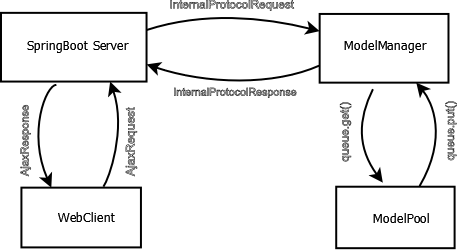
\includegraphics[scale=0.6]{arch} \\
Arhitectura generara a proiectului
\end{tabular}
\end{center}

In diagrama de mai sus observam schematic, abstractizat, principalele componenente ale proiectului si relatiile dintre ele. In continuare descriem in detaliu aceste relatii: 
\begin{itemize}
	\item \textbf{SpringBoot Server} - \textbf{WebUI}, etapa principala din ciclul de viata al proiectului este livrarea codului interfetei clientului, apoi, de interes este interactiunea dintre \textit{WebUI} si server. De obicei fluxul normal este:
	\begin{enumerate}
		\item Utilizatorul selecteaza numarul de fire, modelul antrenat folosit si asteapta producerea rezultatului. In spate, \textit{WebUI} impacheteaza optiunile utilizatorului intr-un pachet \textit{JSON} si trimite prin \textit{AJAX} un request catre server.
		\item \textit{Serverul} primeste requestul de la \textit{WebUI} printr-un endpoint. In functie de optiunile alese, se creeaza un apel catre clasa \textit{ManagerClient} care are rolul de a fi un adaptor intre server si \textit{ModelManager}. 
		\item \textit{Server}-ul impacheteaza intr-un \textit{JSON} lista de comparatori returnata de \textit{ManagerClient} si il trimite \textit{WebUI}-ului.
		\item \textit{WebUI}-ul primeste \textit{response}-ul \textit{AJAX} cu lista de comparatori si initiaza un apel spre modulul de desenare, care creeaza reprezentarea grafica a retelei produse.
	\end{enumerate}
	\item \textbf{SpringBoot Server} - \textbf{ModelManager}, comunicarea dintre aceste componente este, de regula, initializata de \textit{ManagerClient} si cronologic este structurata astfel:
	\begin{enumerate}
		\item \textit{ManagerClient}-ul initiaza o conexiune TCP/IP cu \textit{ModelManager}-ul. Ii trimite acestuia un pachet codificat intr-un protocol propriu ce contine numarul de fire si modelul pe baza caruia sa se genereze comparatorii.
		\item \textit{ModelManagerul}-ul accepta conexiunea de la \textit{ManagerClient}, primeste pachetul, il decodifica si realizeaza un apel catre \textit{ModelThreadPool}, apoi impacheteaza lista de comparatori generata si o trimite inapoi la \textit{ManagerClient}. 
	\end{enumerate}
	\item \textbf{ModelManager} - \textbf{ModelPool}. De la initializare \textit{ModelPool}-ul incarca de pe disc fiecare dintre modele si porneste un thread separat ce le ruleaza. 
	\begin{enumerate}
		\item In functie de modelul ales \textit{ModelManager}-ul realizeaza un apel la metoda respectiva din \textit{ModelPool}.
		\item Prin intermediul unei cozi \textit{thread-safe}, \textit{ModelPool}, semnalizeaza threadul cu modelul respectiv ca trebuie evaluat un nou rezultat. Rezultatul modelului este transmis inapoi prin acelasi mecanism.
	\end{enumerate}
	
\end{itemize}



In continuare dorim sa analizam mai atent structura si modul de functionare al \textit{ModelManager}-ului.

\begin{center}
\begin{tabular}{cc}
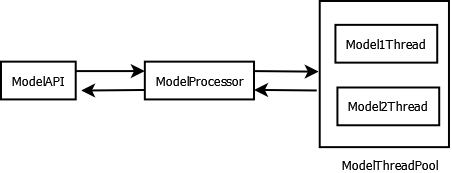
\includegraphics[scale=0.9]{manager_arch} \\
Arhitectura interna a model managerului
\end{tabular}
\end{center}


In diagrama de mai sus sunt expuse principalele submodule ale managerului. Expunem succint scopul fiecarui submodul:
\begin{itemize}
	\item \textit{ModelApi}, reprezinta un server TCP/IP ce ruleaza pe portul \textit{2018}. Comunicarea cu componenta de \textit{ModelManager} se face prin trimiterea de TCP/IP pe acest port.
	\item \textit{ModelProcessor}, decodifica pachetele primite de eventualii utilizatori apeleaza metoda potrivita din urmaorul submodul. \textit{ModelProcessor}-ul are si rolul de a aproxima probabilitatile din lista de comparatori generata de model.
	\item \textit{ModelThreadPool}, incarca de pe disc fiecare dintre modelele salvate si apoi creeaza un thread in care ruleaza fiecare model. Comunicarea dintre threadul principal se face prin intermediul a doua cozi \textit{thread-safe}. Threadul principal pune un coada numarul de fire dorit, iar threadul ce ruleaza modelul respectiv pune in a doua coada lista de comparatori generarata. 
\end{itemize}

\subsection{Arhitectura modelului}

Modelul este un "Neural Turing Machine". Pentru constructia modelului am folosit in spate un framework numit ntm-lasage, optimizat pentru crearea de modele de acest fel. Se abstractizeaza in acest fel detalii de implementare. 

Modelul contine o memorie cu un layout de $1024$x$160$ celule. Ca functie de loss am folosit crossentropia binara, pentru ca intern numerele ce vin ca input in model sunt reprezentate ca siruri binare.

Procesul de backpropagation este abstractizat de model. Actualizarea weighturilor din retea este optimizata cu rmsprop.
Datele de antrenament sunt procesate de retea in batchuri de 1.

Structura inputului retelei este de un vector de 9 elemente ce reprezinta codificarea in binar a numarului de fire din retea. Outputul retelei este un vector tridimensional cu $2*numar\_comparatori$ elemente. Elementele din vector sunt semantic grupate 2 cate 2, codificate ca un sir de biti, si reprezinta pozitiile comparatorilor din retea. 

\subsection{Codul modelului}

\begin{figure}
\centering
\begin{lstlisting}
def model(input_var, batch_size=1, size=8, num_units=100, memory_shape=(1024, 160)):

    l_input = InputLayer((batch_size, None, size + 1), input_var=input_var)
    _, seqlen, _ = l_input.input_var.shape

    memory = Memory(memory_shape, name='memory', 
    	memory_init=lasagne.init.Constant(1e-6), learn_init=False)
    controller = GRUController(l_input, memory_shape=memory_shape,
        num_units=num_units, num_reads=1,
        nonlinearity=lasagne.nonlinearities.rectify,
        name='controller')
    heads = [
        WriteHead(controller, num_shifts=3, memory_shape=memory_shape, 
        	name='write', learn_init=False,
            nonlinearity_key=lasagne.nonlinearities.rectify,
            nonlinearity_add=lasagne.nonlinearities.rectify),
        ReadHead(controller, num_shifts=3, memory_shape=memory_shape, 
        	name='read', learn_init=False,
            nonlinearity_key=lasagne.nonlinearities.rectify)
    ]
    l_ntm = NTMLayer(l_input, memory=memory, controller=controller, heads=heads)

    l_output_reshape = ReshapeLayer(l_ntm, (-1, num_units))
    l_output_dense = DenseLayer(l_output_reshape, num_units=size + 1, 
    	nonlinearity=lasagne.nonlinearities.sigmoid, \
        name='dense')
    l_output = ReshapeLayer(l_output_dense, (batch_size, seqlen, size + 1))

    return l_output, l_ntm

\end{lstlisting}
\caption{Sursa modelului}
\end{figure}

\subsection{Antrenarea modelului}

Modelul ce genereaza retele bubble sorter a fost antrenat pe un set de input 1000 de elemente, pe numere mai mari de atat timpul necesar finalizarii procesului de antrenament devine foarte mare. Datele din setul de antrenament au fost generate conform algoritmului:
\begin{lstlisting}
    def bubble_sorter(n):
        if n <= 1:
            return []

        ret_val = []
        for i in range(0, n - 1):
            ret_val.append((i, i + 1))
        ret_val += self.dummy_sorter(n - 1)
        return ret_val
\end{lstlisting}



si arata astfel pentru un set de antrenament de 5 elemente:

\begin{lstlisting}
[2, [(0, 1)]]
[3, [(0, 1), (1, 2), (0, 1)]]
[4, [(0, 1), (1, 2), (2, 3), (0, 1), 
	(1, 2), (0, 1)]]
[5, [(0, 1), (1, 2), (2, 3), (3, 4), 
	(0, 1), (1, 2), (2, 3), (0, 1), (1, 2), (0, 1)]]
[6, [(0, 1), (1, 2), (2, 3), (3, 4), 
	(4, 5), (0, 1), (1, 2), (2, 3), 
	(3, 4), (0, 1), (1, 2), (2, 3), (0, 1), (1, 2), (0, 1)]]
\end{lstlisting}

Insa date de mai sus reprezinta la nivel abstract inputul si outputul dorit pentru retea. In proiect datele sunt reprezentate in binar ca un sir de 9 biti, iar interschimbarile nu sunt reprezentate explicit ca tuple. Reteaua va produce, practic, o lista de siruri biti ce vor fi grupate, in ordine, 2 cate 2.

Spre exemplu, pentru urmatorul input:

\begin{lstlisting}
numpy.array([[[0, 0, 0, 0, 0, 0, 0, 1, 1]]])
\end{lstlisting}

reprezinta dimensiunea 3, adica reteau va trebui sa genereze setul de comparatori pentru o retea de 3 elemente. Inputul de mai sus a fost testat pe o retea antrenata pe un set de date 1000 elemente, modelul este Bubble Sorter. Outputul produs este urmatorul:
\begin{center}
\begin{multicols}{2}
\begin{lstlisting}
[[[0.000751546365971,
0.000769892576671,
0.000637261131599,
0.000600783421602,
0.12773718494,
0.239040904467,
0.214272843324,
0.370771723772,
0.465849417004],

[9.00920625725e-05,
7.82020981282e-05,
6.5095684253e-05,
6.73165195701e-05,
0.180481531645,
0.244833481652,
0.273710496834,
0.454686659751,
0.496889833317],

[4.46837405637e-05,
3.44817119736e-05,
2.6885035585e-05,
3.21667374046e-05,
0.262205621903,
0.240104608732,
0.341346314965,
0.501759117299,
0.507289515972],

[3.48919682303e-05,
2.59198402876e-05,
1.83589819237e-05,
2.46684454266e-05,
0.330040528556,
0.237285575094,
0.394284580217,
0.525120693702,
0.510196603956],

[3.10455175941e-05,
2.33229850784e-05,
1.51453999616e-05,
2.18735040572e-05,
0.376419535208,
0.237146807326,
0.429571992622,
0.537611938861,
0.511490463268],

[2.89867797738e-05,
2.23753419482e-05,
1.35824510377e-05,
2.04069513415e-05,
0.406359755172,
0.238643669264,
0.452255805808,
0.54490706061,
0.513243797725]]]
\end{lstlisting}
\end{multicols}
\end{center}

-- extinde in sectiune cu `Rezultate Obtinute`
-- adauga schema retelelor obtinute, perechile input-output pentru 3 sample-uri de outputuri
 
Semnificatia fiecarui double din lista este probabilitatea ca bitul respectiv sa fie 1. Acuratetea probabilitatilor se sporeste cu antrenarea sporita a modelului. Intr-un final, se grupeaza 2 cate 2 elementele din lista si se decodifica din binar in decimal.

\subsection{Prezentarea interfetei}

-- pune 1-2-3 screenshoturi
-- vorbeste foarte succint despre fiecare optiune pe care o are utilizatorul

\section{Retele de sortare}

In cadrul acestui capitol prezentam acestui capitol prezentam fundamentele teoretice necesare pentru intelegerea conceptului de \textit{retea de sortare} cat si aplicatiile acestora in practica

\subsection{Prezentare}

O retea de sortare cu $n$ inputuri este o secventa fixa de comparatii si interschimbari (comparatori) ce sorteaza toate inputurile de marime $n$. Deoarece aceeasi secventa de comparatori sorteaza orice secventa de marime $n$, reprezinta un algoritm de sortare independent de date. Asta inseamna ca secventa de comparatii ce se executa nu depinde de inputul primit. Datorita structurii pe care o are o retea de sortare, sunt de preferat in implementarile paralele ale algoritmilor de sortare, precum cele de pe placile grafice.

Motivati de aceste aplicatii in practice, retelele de sortare sunt un subiect important de cercetare inca din 1950. Un interes deosebit il au retelele de sortare optimale, care folosesc numarul minim posibil de comparatori. Generarea retelelor de sortare optimale reprezinta o problema grea de optimizare, investigata pentru prima data de O'Connor si Nelson pentri $4 \leq n \leq 8$. Retelele gasite de cei 2 aveau numarul minim de comparatori pentru $4, 5, 6$ si $8$ inputuri, dara veau nevoie de 2 comparatori in plus pentru $7$ inputuri. Acest rezultata a fost imbunatatit in 1968 de Batcher care a gasit retele minimale pentru $n \leq 8$.

\begin{center}
\begin{figure}

\centering

\begin{sortingnetwork}{4}{5}{1}
\nodelabel{$x_4$, $x_3$, $x_2$, $x_1$}
\nodeconnection{{1,2}}
\nodeconnection{{3,4}}
\nodeconnection{{1,3}}
\nodeconnection{{2,4}}
\nodeconnection{{2,3}}
\nodelabel{$y_4$, $y_3$, $y_2$, $y_1$}
\end{sortingnetwork}
\\
\label{Figura 1}
\caption{O retea de sortare cu 4 inputuri. Valorile de input ${x_1, \ , x_2, \ , x_3, \ , x_4}$ din partea stanga a liniilor orizontale trec printr-o secventa de operatii de comparatii si interschimbari, reprezentate prin linii verticale ce conecteaza perechi de linii orizontale. Fiecare comparator de acest fel isi sorteaza cele doua valori de input, rezultand intr-un final in liniile orizontale ce contin valorile sortate de output ${y_1 \leq y_2 \leq y_3 \leq y_4}$, Aceasta este o retea minimala din punct de vedere a numarului de comparatori folositi.}

\end{figure}
\end{center}

Pana in 2013, se cunosteau retele de sortare minimale doar pentru inputuri $n \leq 8$ (vezi Tabelul 1). In 2013, Valsalam a introdus un articol in care prezinta modalitati de generare a retelelor optimale prin algoritmi evolutivi si reuseste sa obtina noi rezultate pentru $n$ de marime $17 \ , 18, \  19, \ 20, \ , 21$ si $22$. In continuare, gasirea de retele optimale pentru inputuri $n > 8$ ramane o problema deschisa. Un caz particualr de interes este reprezentat de retelele descoperite de Green.

\begin{figure}
\centering
\begin{tabu} to 1.1 \textwidth { | X[0] | X[1] | X[2] |  X[3] | X[4] | X[5] | X[6] | X[7] | X[8] | X[9] | X[10] | X[11] | X[12] | X[13] | X[14] | X[15] | X[16] |}
 \hline
 n & 1 & 2 & 3 & 4 & 5 & 6 & 7 & 8 & 9 & 10 & 11 & 12 & 13 & 14 & 15 & 16\\
 \hline
 C  & 0 & 1 & 3 & 5 & 9 & 12 & 16 & 19 & 25 & 29 & 35 & 39 & 45 & 51 & 56 & 60\\
\hline
\end{tabu}
\caption{Numarul minim de comparatori cunoscut pentru retele de sortare de dimensiune $n \leq 16$. Aceste retele au fost studiate intens, dar s-a dovedit ca doar rezultatele pentru $ n \leq 8$ sunt minimale.}

\end{figure}

\subsection{Principiul 0-1}

\subsubsection{Enunt}
\textit{Principiul 0-1} este o modalitate de verificare a corectitudinii unei retele de sortare. Conform acestuia, o retea de sortare care sorteaza corect orice de secventa de $0$ si $1$, va sorta corect orice secventa de numere.

\subsubsection{Demonstratie}
\textbf{Lemma:} Presupunem $f$ o functie monotona, crescatoare. Atunci, daca o retea mapeaza $x_1$, $x_2$,...,$x_n$ la $y_1$, $y_2$,...$y_n$, va mapa $f(x_1)$, $f(x_2)$,..., $f(x_n)$ la $f(y_1)$, $f(y_2)$,...,$f(y_n)$. 

\textbf{Demonstratie:} Prin inductie la numarul de comparatori din retea folosind:
\begin{tightcenter} 
 $f(min(a, b)) = min(f(a), f(b))$\\
 $f(max(a, b)) = max(f(a), f(b))$\\
\end{tightcenter}

Sa presupunem ca o \textit{retea} nu este retea de sortare. Atunci, va mapa valorile $x_1$, $x_2$,...,$x_n$ arbitrare, la $y_1$, $y_2$,..., $y_n$. Unde $y_i > y_{i+1}$ pentru $1 \leq i  < n$. Presupunem $f(x) = 1$ daca si numai daca $x \geq y_i$, $0$ altfel. Reteaua va mapa $f(x_1)$, $f(x_2)$,..., $f(x_n)$ la $f(y_1)$, ..., $f(y_i)=1$, $f(y_{i+1})=0$, ..., $f(y_n)$. Astfel, reteaua nu va sorta toate inputurile de tipul $0-1$.



\subsection{Generarea retelelor de sortare folosind algoritmi evolutivi}

In acest subcapitol descriem succint modalitatea de generare a retelelor de sortare optimale folosind algorimti evolutivi. Motivul pentru care am ales sa aducem in lumina si aceasta abordare este ca, proflema fiind una dificila de rezolvat prin metode imperative, s-a incercat abordarea acesteia prin metode evolutive, iar rezultatele sunt surprinzatoare.

In principal, vom descrie metoda introdusa de \textit{Valsalam} si \textit{Miikkulainen}, (SENSO[15]). 

\subsubsection{Reprezentarea functiilor booleane}

Folosind principiul \textit{0-1} descris mai sus, putem exprima inputul unei retele de sortare ca variabile booleane, iar outputul retelei ca functii de aceste variabile. Astfel, problema gasirii comparatorilor pentru o retea de sortare se reduce la a numara firele ce au ca input valoarea $1$ si a seta outputul firelor de output \textit{de mai jos} la valoarea $1$, iar outputul firelor ramase la $0$. Deoarece aceste functii sunt implementate de comparatorii din retea, problema gasirii unei retele de sortare se poate reduce la problema gasirii unei secvente de comparatori care ii genereaza functiile de output.

\subsubsection{Simetrii in retele de sortare}
O simetrie intr-o retea de sortare este o operatie pe setul de functii de output al retelei care nu afecteaza outputul retelei. Valsalam defineste formal operatie de simetrie  $\sigma_i$ pentru $1 \leq i \leq \mid\frac{n}{2}|$ care opereaza pe setul de functii de output din retea prin interschimbarea functiei $f_i$ si dualei $f_{n+1-i}$, interschimband conjunctia si disjuctia dintre ele. Compozitia simetriilor este tot o simetrie, fiind inchisa la compozitie. 
\subsubsection{Minimizarea numarului de comparatori necesari}

-- to do

\subsubsection{Evoluarea retelelor minimale}

Valsalam initializeaza evolutia cu o populatie de solutii produse de algoritmul greedy. Valoarea de \textit{fitness} a fiecarei solutii este $-1 \  \cdot $ \texttt{numarul de comparatori}, pentru ca imbunatatirea \textit{fitness}-ului sa rezulte intr-un numar mai mic de comparatori generati. La fiecare noua generatie, selectia se face prin metoda \textit{turneu} pe baza valorii de \textit{fitness} pentru a selecta indivizii din populatie pentru reproducere. La reproducere se muteaza reteaua parinte si se creeaza o retea de \textit{offspring} in doi pasi:
\begin{enumerate}
	\item Un comparator este ales in mod aleator din retea si apoi se trunchiaza reteaua dupa el, eliminand comparatorii ce urmeaza dupa el.
	\item Algoritmul greedy este folosit pentru a adauga noi comparatori construind o noua retea. Pentru ca algoritmul greedy alege un comparator cu cea mai mare utilitate in mod aleator, aceasta mutatie exploreaza o noua combinatie de comparatori ce ar putea fi mult mai folositori decat comparatorul parinte.
\end{enumerate}
Aceasta abordare restrange spatiul de cautare la comparatorii generati de algorimtul greedy.
SENSO[15] a fost rulat pe o populatie de marime 200 pentru 500 de generatii ca sa evolueze de retele de sortare optimale. La fiecare generatie, au selectate cele 100 de retele cu numarul minimal de comparatori pentru a estima modelul. Acelasi set de retele a fost copiat la urmatoarea generatie, fara modificari, ....

Experimentul de mai sus a fost repetat de $20$ de ori pentru fiecare varianta a algoritmului greedy si pentru fiecare input $n \leq 23$

Numarul de comparatori gasit de SENSO in corespondenta cu marimea reteli este reprezentat in figura de mai jos.



\subsection{Retelele optimale}

\subsubsection{Prezentare}
In aceasta sectiune a lucrarii dorim sa amintim despre \textit{retelele lui Green}, intrucat folosind metoda lui \textit{Green} de construire a retelelor obtinem numarul minimal de comparatori.

Mai jos afisam rezultatul metodei lui \textit{Green} pentru o retea de marime $16$:

\begin{figure}
\centering
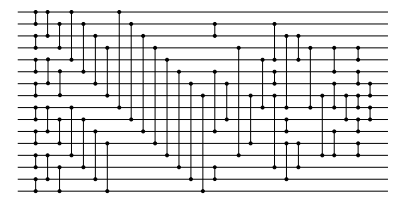
\includegraphics[scale=1.0]{green_net}
\\
\caption{Reteaua de comparatori a lui green pentru un input $n = 16$}
\end{figure}

Acesta retea are $60$ de comparatori, care reprezinta cea mai mica valoare cunoscuta pentru o retea cu 16 inputuri[16][17]. Comparatorii dintr-o astfel de retea sunt simetric aranjati de la axa orizontala pana in mijlocul retelei. Acest tip de retele au reprezentat pentru unii cercetatorii obiectiv de studiu pentru dezvoltarea algoritmilor evolutivi care genereaza retele de sortare. 

\subsection{Metode imperative de generare a retelelor de sortare}

Exista mai multe metode imperative pentru a genera o retea de sortare. Cele mai usoare modalitati sunt de a generea o 
retea bazata pe algoritmii de sortare bubble sort si insertion sort. In cazul primei optiuni se adauga un comparator intre
firele $0$ si $1$, $1$ si $2$, ..., $n-1$ si $n$. Se reaia procesul de creere a comparatorilor inserand un comparator intre $0$ si $1$, ..., $n-2$ si $n-1$. Se repeta aceasta procedura de creere a comparatorilor pana la pasul in care inseram un singur comparator intre firele $0$ si $1$.

In cazul unei insertion sorting network, o retea bazata pe insertion sort procesul este similar, singura diferenta este ca buclele de creare a comparatorilor sunt in ordine inversa fata de metoda precedenta. Astfel, prima data se creeaza un comparator 
intre firul $0$ si $1$. Se creeaza un comparator intre $0$ si $1$, $2$. Pana cand se ajunge la pasul in care se generaza un comparator intre $0$ si $1$, ..., $n-1$ si $n$. 

Un exemplu de bubble sorting network:

\begin{figure}
\centering
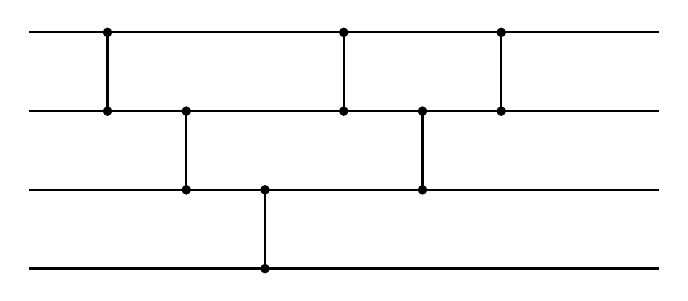
\begin{tikzpicture}
%\fill [gray!15] (1.5,1.5) -- (2.5,1.5) -- (2.5,2.5) -- (1.5,2.5) -- cycle;
\foreach \a in {1,...,4}
  \draw[thick] (0,\a) -- ++(8,0);
\foreach \x in {{1,4},{1,3}, {2,3},{2,2},{3,2},{3,1},{4,4},{4,3},{5,3},{5, 2}, {6, 3}, {6, 4}}
  \filldraw (\x) circle (1.5pt);
\draw[thick] (1,4) -- (1,3);
\draw[thick] (2,3) -- (2,2);
\draw[thick] (3,2) -- (3,1);
\draw[thick] (4,4) -- (4,3);
\draw[thick] (5,3) -- (5,2);
\draw[thick] (6,4) -- (6,3);
\end{tikzpicture}
\caption{Retea de sortata generata pe baza algoritmului \textit{Bubble Sort} cu $n=4$ inputuri. }
\end{figure}

Un exemplu de insertion sorting network:

\begin{figure}
\centering
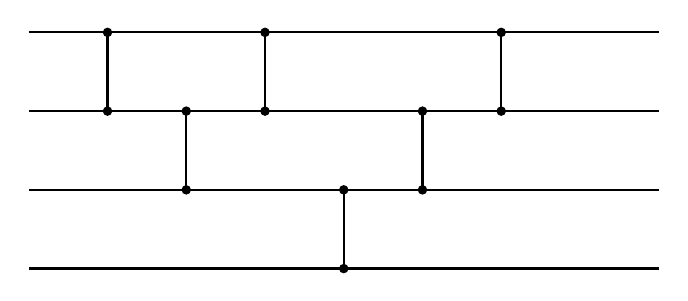
\begin{tikzpicture}
%\fill [gray!15] (1.5,1.5) -- (2.5,1.5) -- (2.5,2.5) -- (1.5,2.5) -- cycle;
\foreach \a in {1,...,4}
  \draw[thick] (0,\a) -- ++(8,0);
\foreach \x in {{1,4},{1,3}, {3,4},{3,3},{2,3},{2,2},{4,2},{4,1},{5,3},{5, 2}, {6, 3}, {6, 4}}
  \filldraw (\x) circle (1.5pt);
\draw[thick] (1,4) -- (1,3);
\draw[thick] (3,4) -- (3,3);
\draw[thick] (2,3) -- (2,2);
\draw[thick] (4,2) -- (4,1);
\draw[thick] (5,3) -- (5,2);
\draw[thick] (6,4) -- (6,3);
\end{tikzpicture}
\caption{Retea de sortare generata pe baza algoritmului \textit{Insertion Sort} pentru $n=4$ inputuri.}
\end{figure}

Algoritmul imperativ pe care l-am folosit pentru a genera un bubble sorting network este:
\begin{lstlisting}
    def bubble_sorter(n):
        if n <= 1:
            return []

        ret_val = []
        for i in range(0, n - 1):
            ret_val.append((i, i + 1))
        ret_val += self.dummy_sorter(n - 1)
        return ret_val
\end{lstlisting}
Pentru un numar de fire dat, $n$, generam lista de comparatori, adica conexiunile dintre firele din retea.
%\break

    Aceste arhitecturi de retele de sortare nu sunt optimale si vor sorta un sir de numere ca input in timp
$O(n^2)$. Retelele optimale si cele mai des folosite in practica sunt bazate pe algoritmul bitonic sort, acestea ating complexitate de $O(nlog^2(n))$. Insa motivul pentru care am prezentat bubble sorting network si insertion sorting network este
ca bazandu-ne pe acesti algoritmi am generat datele de antrenament pentru modelul dezvoltat. Motivatia ar fi ca, cel putin din experimentele realizate in cadrul acestui proiect, este mai usor de antrenat un model care sa produca date relevante atunci cand primeste date de antrenament generate pe baza acestor algoritmi.

\subsection{Aplicatii}
Cea mai la indemana aplicatie in practica a retelelor de sortare o reprezinta sortarea pe placile grafice. Placile grafice dispozitive orientate puternic spre paralelizarea instructiunilor, pe arhitectura \textit{single-instruction, multiple data (SIMD}. Si avand in vedere si ca placile grafice depasesc in performanta CPU-ul cand vine vorba de algoritmi cu limita de memorie si timp de calcul, retelele de sortare devin o optiune eficienta.


\section{Retele neuronale, prezentare}

Retelele neuronale reprezinta o ramura a inteligentei artificiale. Sunt modele abstracte ce incearca sa simuleze creierul uman
in modul de intercationare cu natura. O retea neuronala este compusa din neuroni artificiali. Neuronii artificiali din retea sunt dispusi pe mai multe straturi. Din exterior le putem vedea ca pe un black box conectat la un strat de neuroni de input, responabil de preluarea inputlui si la un strat de neuroni de output, responsabil pentru a genera outputul. In functie de neuronii din stratul de output care se vor activa se decodifica rezultatul produs de retea.

\subsection{Arhitecturi de retele neuronale}
Retelele neuronale convolutionale sunt modele simple, proiectate sa primeasca un set de input fix si sa produca un set output output de marime fixa. In practica, acest tip de retele sunt ideale pentru computer vision. Sunt mult mai eficiente din punct de vedere al resurselor consumate la sarcini precum recunoasterea de obiecte in imagini. 

Retelele neuronale recurente se deosebesc de cele convolutionale prin posibilitatea de a primi un set de input variabil si a produce un set de output variabil. In practica se folosesc la procesarea limbajului natural. Acest tip de retele neuronale sunt ideale si pentru rezolvarea problemei de generare a retelelor de sortare, intrucat putem codifica numarul de fire din retea ca o secventa de lungime variabila, iar rezultatul, respectiv setul de comparatori pentru numarul de fire dat poate varia. Pe langa aceste considerente, acest tip de retele contin si o memorie atasata.

Un caz particular de retele neuronale recurente sunt *masinile turing neurale*. Acestea fiind optimizate in a invata algoritmi imperativi simpli. Un exemplu ar fi problema sortarii, rezolvata in mod traditional cu un algoritm imperativ poate fi rezolvata folosind acest tip de retele. Pentru aceasta, reteaua va primi ca input tuple de forma $(X, Y)$. Unde $X$ reprezinta un sir de numere aflate in ordine random, iar $Y$ reprezinta varianta sortata a sirului $X$ cu un algoritm imperativ de sortare. Odata antrenata pe un set suficient de mare de date de acest fel, modelul va invata practic sa aplice algoritmul de sortare folosit pe componenta $Y$. 

Motivul prezentarii scenariului de mai sus este ca hiperparametrii si structura straturilor de neuroni dintr-o retea de neuronala folosita la sortarea de numere sunt similari in proportie foarte mare cu cei din reteaua proiectata sa genereze retele de sortare.

\subsection{Neural Turing Machine (NTM)}

Retelele NTM fac partea din clasa retelelor neuronale recurente si sunt introduse relativ recent. Au fost introduse intr-un articol publicat de Alex Graves in 2014. Acest model de retea neuronala combinata capacitatea de pattern matching a retelelor neuronale cu capacitatea algoritmica a calculatoarelor programabile. Mai exact, putem folosi acest model de retea pentru a invata algoritmti simpli. In paperul introdus de Graves sunt aduse rezultate pentru algoritmi de copiere a unui sir sau sortare. Aceste aspecte ne inspira o probabilitate mare ca o retea bazata pe acest model poate produce rezultate multumitoare pentro problema abordata.

\subsubsection{Descriere}

Neural Turing Machines sunt inspirate din doua lumi: Machine Learning si Teoria Computabilitatii. Prima le permite calculatoarelor sa realizeze taskuri care, desi pentru oameni sunt usoare, se credeau grele pentru calculatoare, precum computer vision. A doua defineste formal lucrurile de care este capabil un calculator. 

Legatura dintre inteligenta artificiala si teoria computatiei in 1940. Modelul introdus de el, Masina Turing, e un model computational clasic care opereaza pe o banda de memorie infinita si un cap care poate sa scrie sau sa citeasca. Pe baza acestor aceste rezultate se inspira si Neural Turing Machines.

Un exemplu de NTM desfasurat in timp:


\begin{figure}
\centering
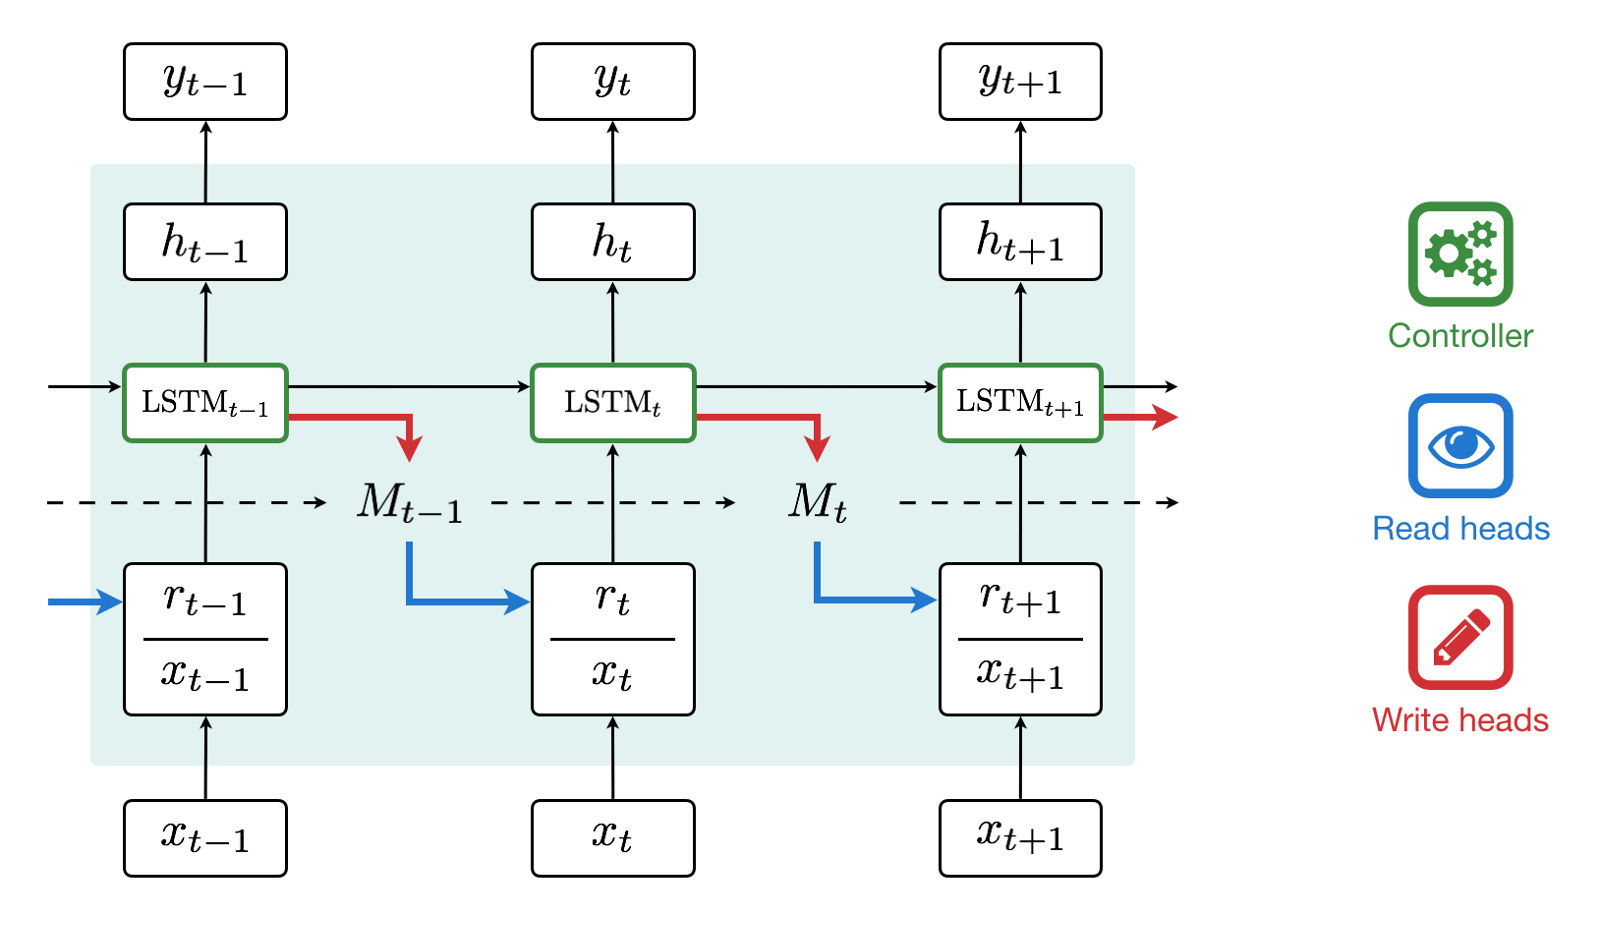
\includegraphics[scale=0.2]{ntm}
\\
\caption{Arhitectura unui Neural Turing Machine. Sursa: \texttt{https://medium.com/snips-ai/
ntm-lasagne-a-library-for-neural-turing-machines
-in-lasagne-2cdce6837315}}
\end{figure}

-- adauga descriere exhaustiva la diagarama

Componenta de controller din cadrul unui Neural Turing Machine este o retea neuronala care pune la dispozitie reprezentarea interna a inputului care este folosit de capetele de scriere si citire ca sa poate interactiona cu memoria. Reprezentarea aceasta nu este identica cu cea stocata in memorie. Tipul de controler pe care il alegem reprezinta cea mai semnificativa alegere arhitecturala. Controllerul poate fi fie o retea feed-forward, fie o retea recurenta.

Capetele de scriere si citire sunt singurele componente din cadrul unui Neural Turing Machine care interactioneaza in mod direct cu memoria. Intern, comportamentul fiecarui dintre capete este controlat de vectorul de weighturi care este actualizat la fiecare pas in timp. Fiecare weight din vector corespunde cu gradul de interactiune cu fiecare celula din memorie. Un weight de 1 focuseaza atentia NTM-ului spre celula respectiva.

Reprezentare vizuala a notiunilor descrise mai sus:

\begin{figure}
\centering
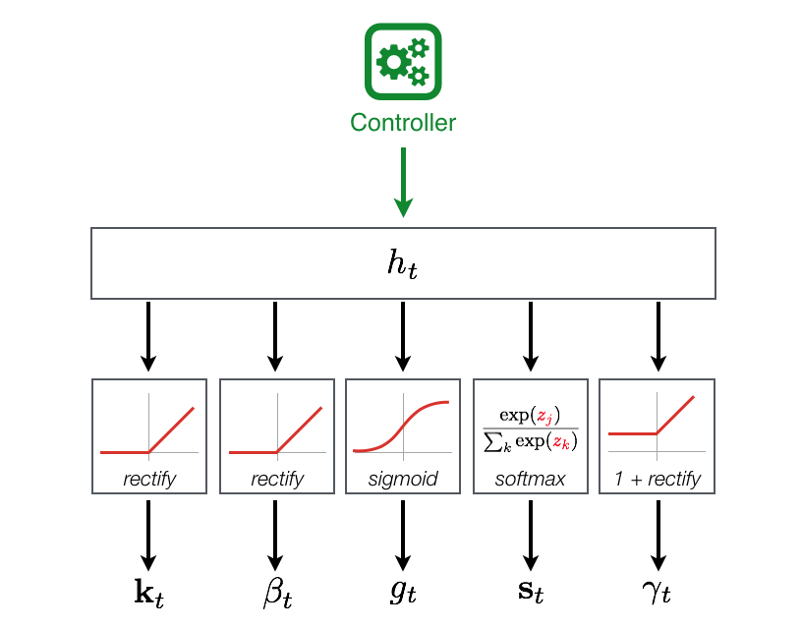
\includegraphics[scale=0.3]{rw_head}
\\
\caption{Arhitectura capului de scriere/citire a unui \textit{Neural Turing Machine}. Sursa: \texttt{https://medium.com/snips-ai/
ntm-lasagne-a-library-for-neural-turing-machines
-in-lasagne-2cdce6837315}}
\end{figure}

\subsubsection{Aplicatii}

-- descriere aplicatii algortimi paraleli de sortare
-- utilizare pe GPU
-- utilizare pe CPU

\section{Tehnologii folosite}

In cadrul proiectului am facut uz de o serie de frameworkuri si biblioteci pentru a fi scutiti de unele detalii de implementare. In aceasta sectiune vom prezenta pe scurt tehnologiile principale folosite.

\subsection{NTMLasagne}

NTMLasagne este frameworkul pe care l-am folosit in proiect ca sa creem modelul. Pe scurt, este un wrapper peste Lasagne  ce ne permite sa creeam "Neural Turing Machines" intr-un mod simplificat, abstractizand detalii de implementare. Ne sunt puse module pentru stratul NTM (en. NTMLayer) unde toate componentele precum capetele de scriere, controllerul si memoria pot fi customizate. In cadrul acestui proiect am ales sa nu customizam niciuna dintre componente. In schimb, le-am folosit pe cele default oferite de framework.

Motivatia din spatele alegerii acestui framework este, chiar daca documentatia este relativ putina, comunitatea puternica din spatele proiectului si faptul ca procesul de dezvoltare este activ.


\subsection{Lasagne}

Lasagne este o biblioteca minimalista folosita pentru construirea de retele neuronale. Permite construire de retele feed-forward, cat si de retele convolutionale, ofera implementari pentru metode de optimizare folosite des (i.e. ADAM si RMSProp). De asemenea, modele construite in Lasagne pot fi antrenate fie pe CPU sau GPU pentru ca biblioteca foloseste Theano in spate.


\subsection{Theano}

Theano este o biblioteca de python ce permite definirea si optimizarea de expresii matematice ce contin array-uri multidimensionale intr-un mod eficient. Chiar daca in momentul de fata Tensorflow este alegerea facuta de majoritatea proiectelor, theano este folosit de cele 2 biblioteci specificate anterior si este in general mai flexibil.

\subsection{Python}

Python este un limbaj de scripting, multi paradigma. Motivul pentru care am ales sa implementam modelul in python este sintaxa usoara, suportul mare pentru biblioteci si frameworkuri de deep learning, atat ca documentatie, cat si ca implementari efective. 

De asemenea componenta de "model manager" care ruleaza intr-un thread fiecare model este scrisa in python.


\subsection{Java}

Java este un limbaj de programare orientat-obiect, puternic tipizat, conceput de către James Gosling la Sun Microsystems (acum filială Oracle) la începutul anilor ʼ90, fiind lansat în 1995. Cele mai multe aplicații distribuite sunt scrise în Java, iar noile evoluții tehnologice permit utilizarea sa și pe dispozitive mobile gen telefon, agenda electronică, palmtop etc. În felul acesta se creează o platformă unică, la nivelul programatorului, deasupra unui mediu eterogen extrem de diversificat. Acesta este utilizat în prezent cu succes și pentru programarea aplicațiilor destinate intranet-urilor

In proiect, Java a fost folosit la crearea backendului pentru interfata web. Motivatia alegerii este experienta puternica anterioara a autorului.

\subsection{Spring Boot}

In cadrul proiectului am pus la dispozitie si o interfata web in care se afiseaza reprezentarea vizuala a retelei generate de modelul ales de utilizator. Backendul acestei interfete este scris in Java si are in spate Spring Boot.

Pe scurt Spring Boot este frameworkul web pe care l-am folosit pentru a scrie serverul proiectului. Ni se pune la dispozitie posibilitatea de a scrie relativ usor o aplicatie web pe arhitectura MVC. 


Motivul pentru care s-a ales Spring Boot in pofida unui alt framework web de Java este documentatia vasta si experienta anterioara a autorului cu aceasta tehnologie.

\subsection{RaphaelJS}

RaphaelJS reprezinta biblioteca de javascript folosita pentru desenarea in browser retelei generate de modelul ales de utilizator. RaphaelJS este un wrapper peste WebGL cu un API relativ usor de folosit.


\subsection{Twitter Bootstrap}

Twitter Bootstrap este un framework web pentru componenta de frontend. Se pun la dispozitie mai multe clase CSS pentru crearea de componente vizuale precum butoane, bare de meniu, cat si un mecanism specific de de pozitionare a continutului.

Motivul pentru care am introdus si aceasta dependinta in stiva de tehnologii folosita in proiect si nu am creat toata interfata in RaphaelJS este performanta. Desenarea intregului design si implementarea si mecanicilor din spate (precum gestionarea apasarilor de buton) ar fi fost remarcabil mai lenta.

\pagebreak

\section{Concluzii}

 In momentul de fata, cele doua modele antrenate, nu produc rezultate multumitoare, nu sunt capabile sa genereze comparatori pentru retele de dimensiuni mari. Optimizarea acestor modele pentru inputuri $N>4$ poate reprezenta o directie de viitor pentru proiect. Acest lucru ar putea fi realizat printr-o metoda introdusa relativ recent (\textit{Mai 2018})[18].

Readucem in atentie ca aceasta lucrare contine un element de noutate, intrucat aceasta abordarea de a genera retele de sortare folosind \textit{deeplearning} nu a mai fost atinsa pana in acest moment. 
  
 


\pagebreak
\begin{thebibliography}{12}
\bibitem{l1} 
 https://github.com/primaryobjects/nnsorting

\bibitem{l2} 
$https://github.com/drforester/Sequence\_to\_Sequence\_Sorting$

\bibitem{l3} 
 https://github.com/aditya-prasad/dnnet

\bibitem{l4} 
 https://adventuresinevolutionblog.wordpress.com/2016/09/17/minimal-sorting-networks/

\bibitem{l5} 
 http://aclweb.org/anthology/I17-3017


\bibitem{l6} 
 http://psycnet.apa.org/record/1999-02657-007 -- Seven times seven is about fifty

\bibitem{l7} 
 https://www.sciencedirect.com/science/article/pii/S0020025512007670

\bibitem{l8} 
 https://github.com/apache/incubator-mxnet/tree/master/example/bi-lstm-sort -- sort numbers using lstm architecture 

\bibitem{l9} 
 $https://rylanschaeffer.github.io/content/research/neural\_turing\_machine/main.html$

\bibitem{l10} 
 https://github.com/carpedm20/NTM-tensorflow

\bibitem{l11} 
 http://www.robots.ox.ac.uk/~tvg/publications/talks/NeuralTuringMachines.pdf

\bibitem{l12} 
 https://medium.com/snips-ai/ntm-lasagne-a-library-for-neural-turing-machines-in-lasagne-2cdce6837315

\bibitem{l13}
 http://www.iti.fh-flensburg.de/lang/algorithmen/sortieren/networks/nulleinsen.htm

\bibitem{l14}
 http://www.cs.tau.ac.il/~zwick/Adv-Alg-2015/Sorting-Networks.pdf

\bibitem{valsalam2013}    
 Valsalam, Vinod K. and Miikkulainen, Risto
 \newblock Using Symmetry and Evolutionary Search to Minimize Sorting Networks
 \newblock \emph{J. Mach. Learn. Res.}, 14\penalty0 (1): \penalty0 303--331, feb 2013

\bibitem{knuth1998}
 D. E. Knuth. Art of Computer Programming: Sorting and Searching, volumul 3, capitolul 5, paginile
 219–229. Addison-Wesley Professional, 2 edition, April 1998

\bibitem{green1972}
 M. W. Green. Some improvements in non-adaptive sorting algorithms. In Proceedings of the Sixth
 Annual Princeton Conference on Information Sciences and Systems, paginile 387–391, 1972.

\bibitem{rubix}
 Stephen McAleer, Forest Agostinelli, Alexander Shmakov, Pierre Baldi
 Solving the Rubik's Cube Without Human Knowledge, 18 Mai 2018

\bibitem{graves_ntm}
 Alex Graves, Greg Wayne, Ivo Danihelka
 Neural Turing Machines, 20 Oct 2014
 
\bibitem{gpu}
 \newblock Peter Kipfer, Rüdiger Westermann
 \newblock Improved GPU Sorting,
 \newblock $https://developer.nvidia.com/gpugems/GPUGems2/gpugems2\_chapter46.html$, Aprilie 2005
 


\end{thebibliography}

\end{document}